\documentclass{proc}
\usepackage[utf8]{inputenc}
\usepackage[francais]{babel}
\usepackage{graphicx}
\usepackage{amsmath}
\usepackage{float}
\usepackage{hyperref}
\usepackage{listings}

\title{Rapport du TP3 \\ IFT3913}

\author{Yalin Mo (20199655) \\ Vennila Sooben (20235256)}
\date{\today}

\begin{document}

\maketitle

\section{Introduction}
% Présentation du problème et des objectifs du travail pratique
Dans cette section, nous présentons l'étude des métriques logicielles de JFreeChart qui est une bibliothèque de graphiques pour Java créée par Dave Gilbert il y a 23 ans \cite{JFreeChart}. L'objectif de ce travail pratique est d'analyser les métriques TLOC (Nombre de lignes de code non-vides qui ne sont pas de commentaires), WMC (Weighted Methods per Class), et TASSERT (nombre d'assertions) des classes de l'application. Cette analyse vise à évaluer la qualité du logiciel et à comprendre les corrélations entre ces métriques. Nous procéderons avec en premier lei une visualisation à l'aide de diagrammes à moustaches. Puis, nous enchaînerons avec une étude de corrélation avec des calculs de coefficients et des diagrammes. Nous finirons avec une analyse des données obtenues pour ainsi proposer une conclusion réfléchie de notre cas d'études.
\vspace{-20px}
\section{Tâche 1: Visualisation des Métriques avec Excel}
\subsection{Création des Diagrammes à Moustaches}
% Description de la création des boîtes à moustaches dans Excel
% Inclusion des diagrammes à moustaches générés dans Excel
Pour visualiser les métriques, nous avons créé des boîtes à moustaches à l'aide d'Excel. \\Les diagrammes montrent les valeurs suivantes :
\\
\begin{itemize}
\item{TLOC: }
\begin{itemize}
    \item Median: 83
    \item Limite Supérieur: 125
    \item Limite Inférieure: 47
    \begin{figure}[H]
    \centering
    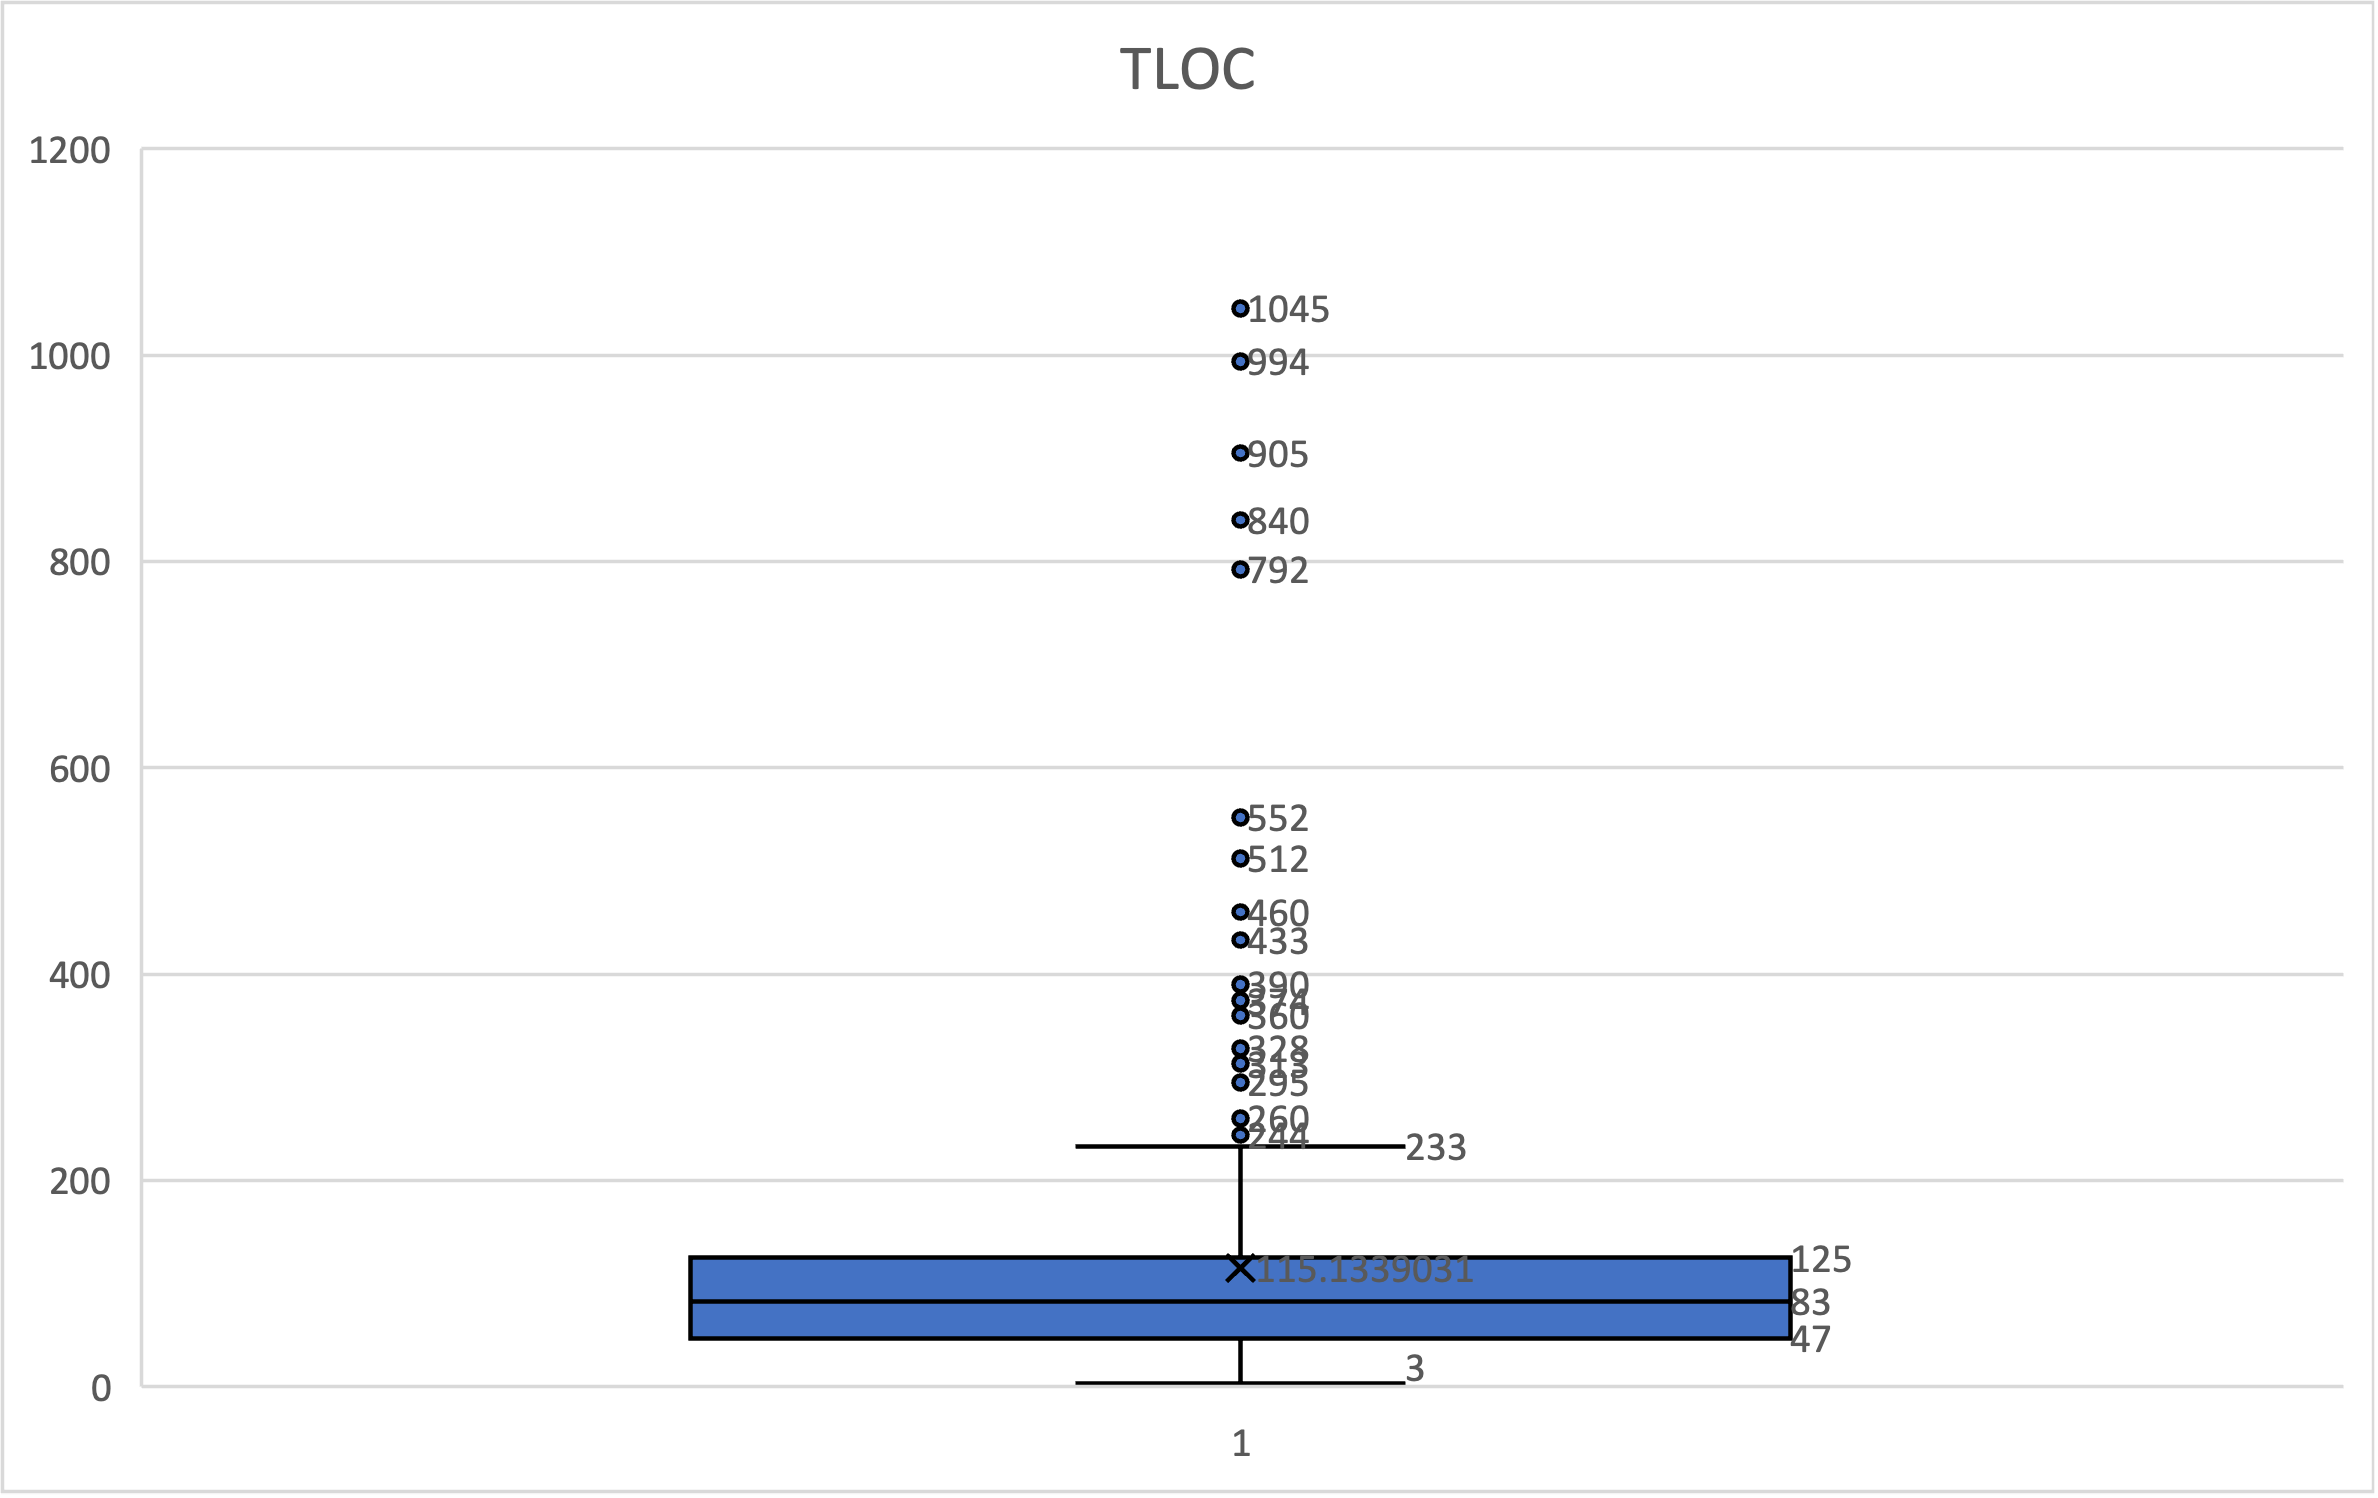
\includegraphics[width=0.5\textwidth]{images/TLOC.png}
    \caption{Boîte à moustaches TLOC}
    \label{fig:TLOC.png}
    \end{figure}
\end{itemize}
\vspace{8px}

\item{WMC}
\begin{itemize}
    \item Median: 9
    \item Limite Supérieur: 12
    \item Limite Inférieure: 8
    \begin{figure}[H]
    \centering
    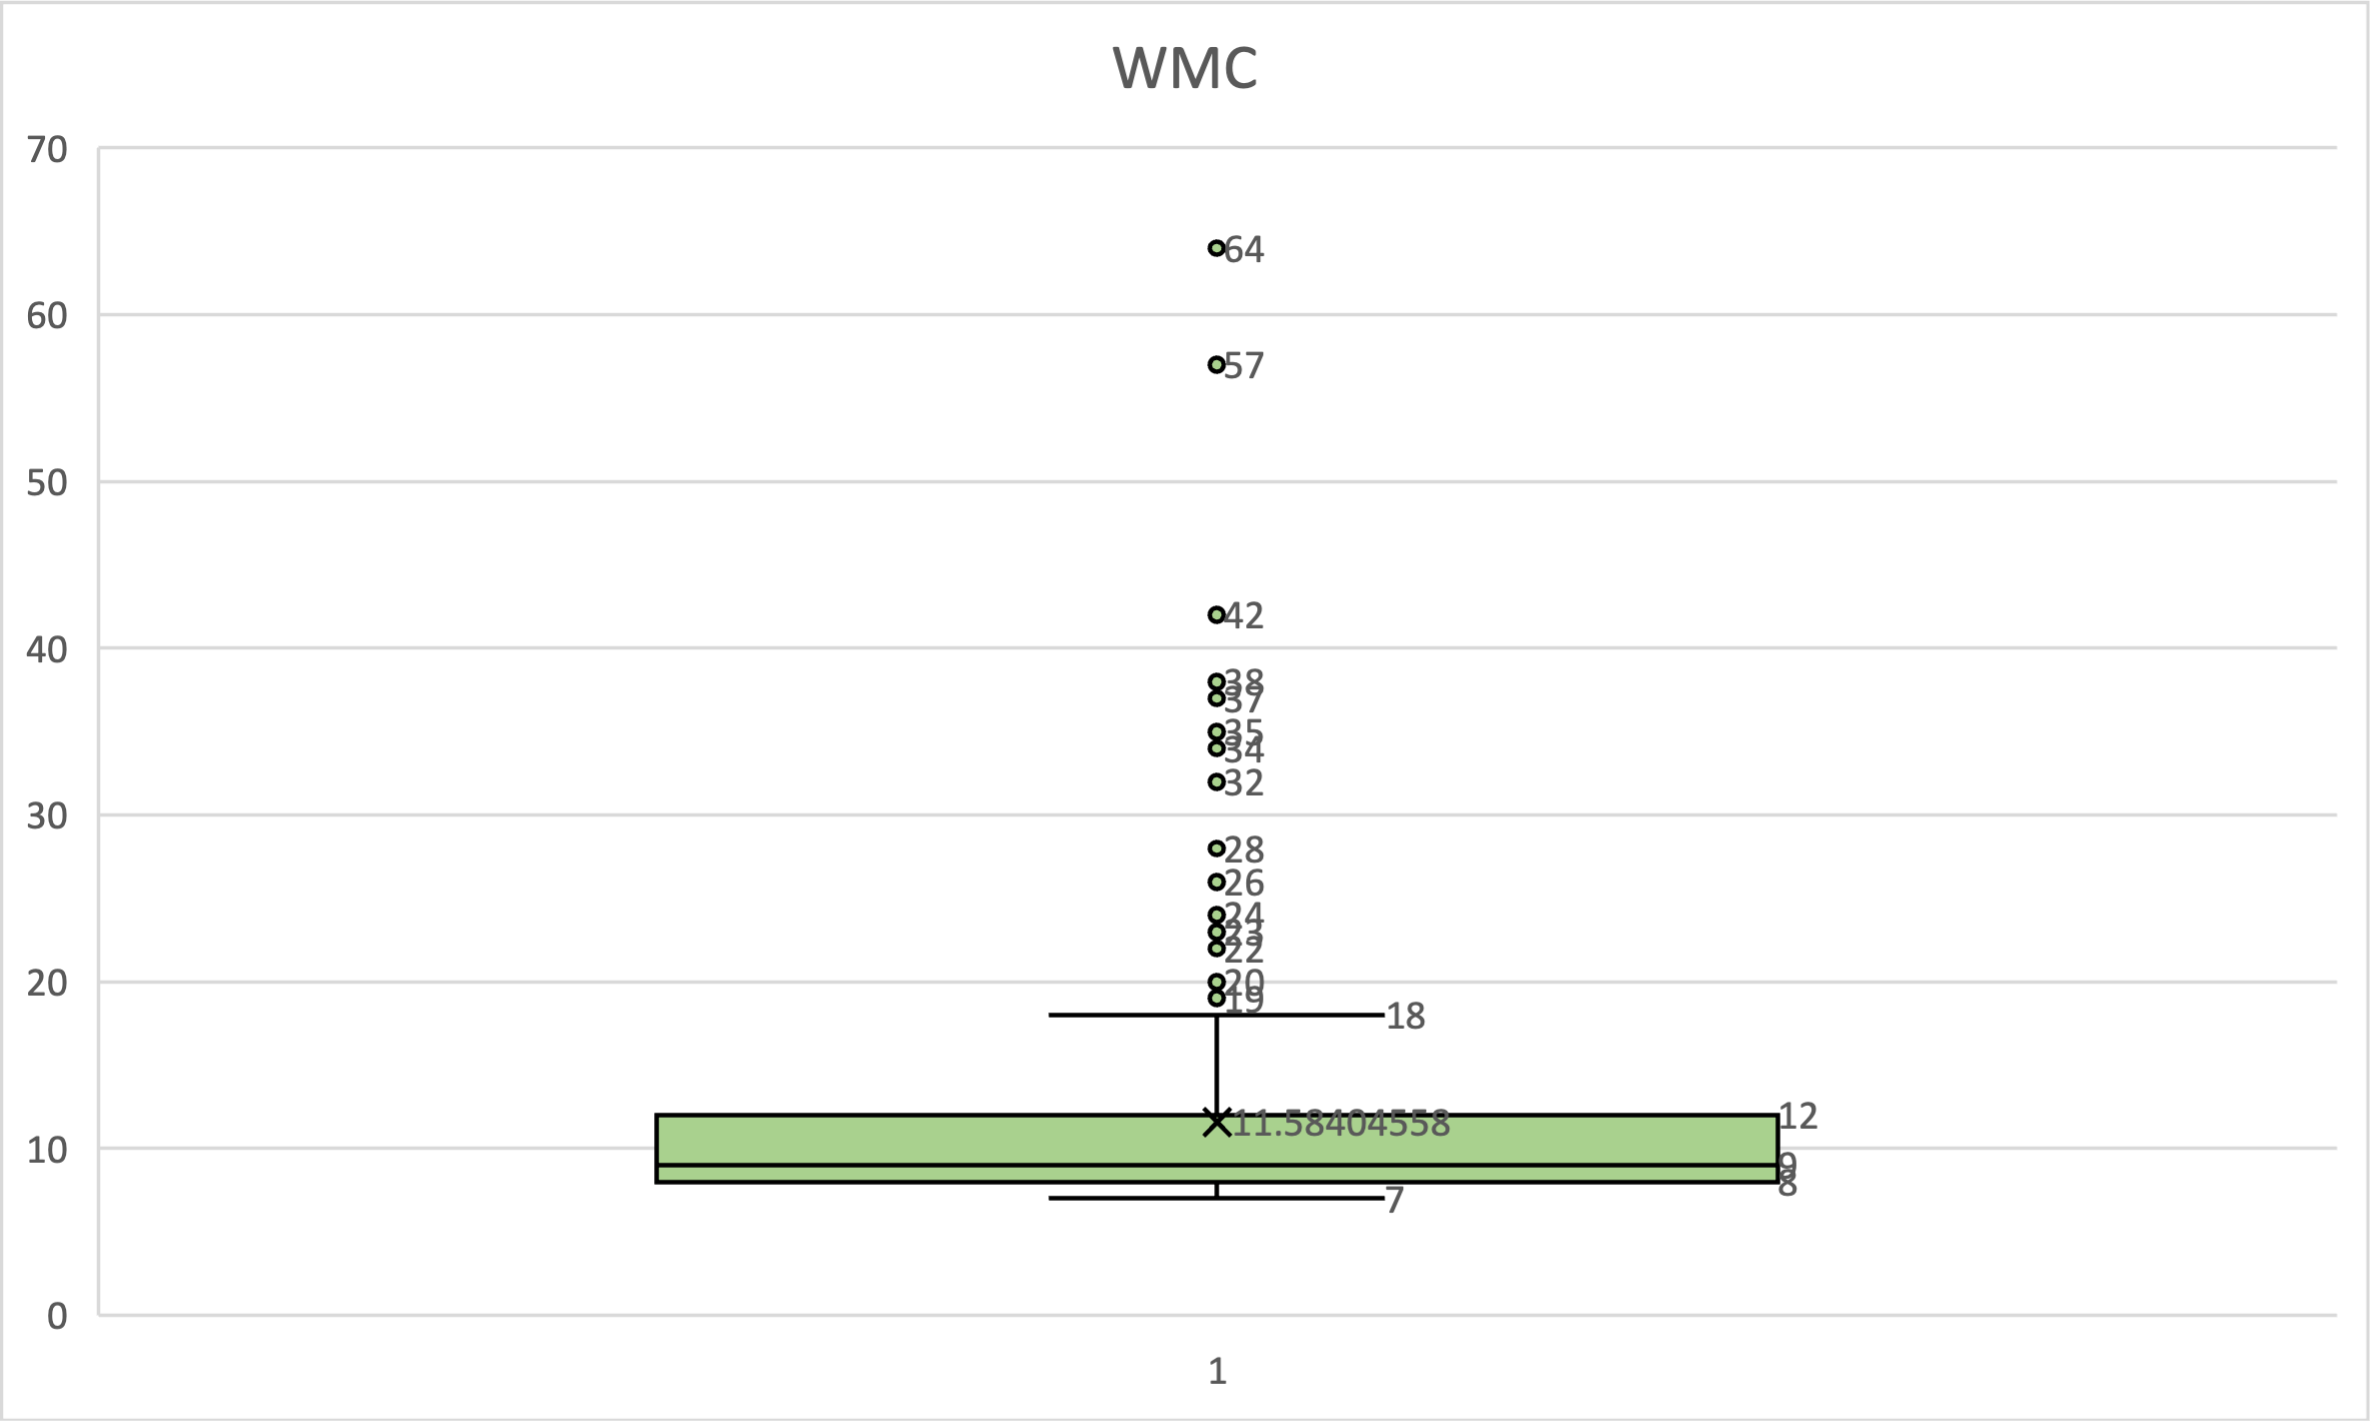
\includegraphics[width=0.5\textwidth]{images/WMC.png}
    \caption{Boîte à moustaches WMC}
    \label{fig:WMC.png}
    \end{figure}
\end{itemize}

\item{TASSERT}
\begin{itemize}
    \item Median: 17
    \item Limite Supérieur: 21
    \item Limite Inférieure: 10
    \begin{figure}[H]
    \centering
    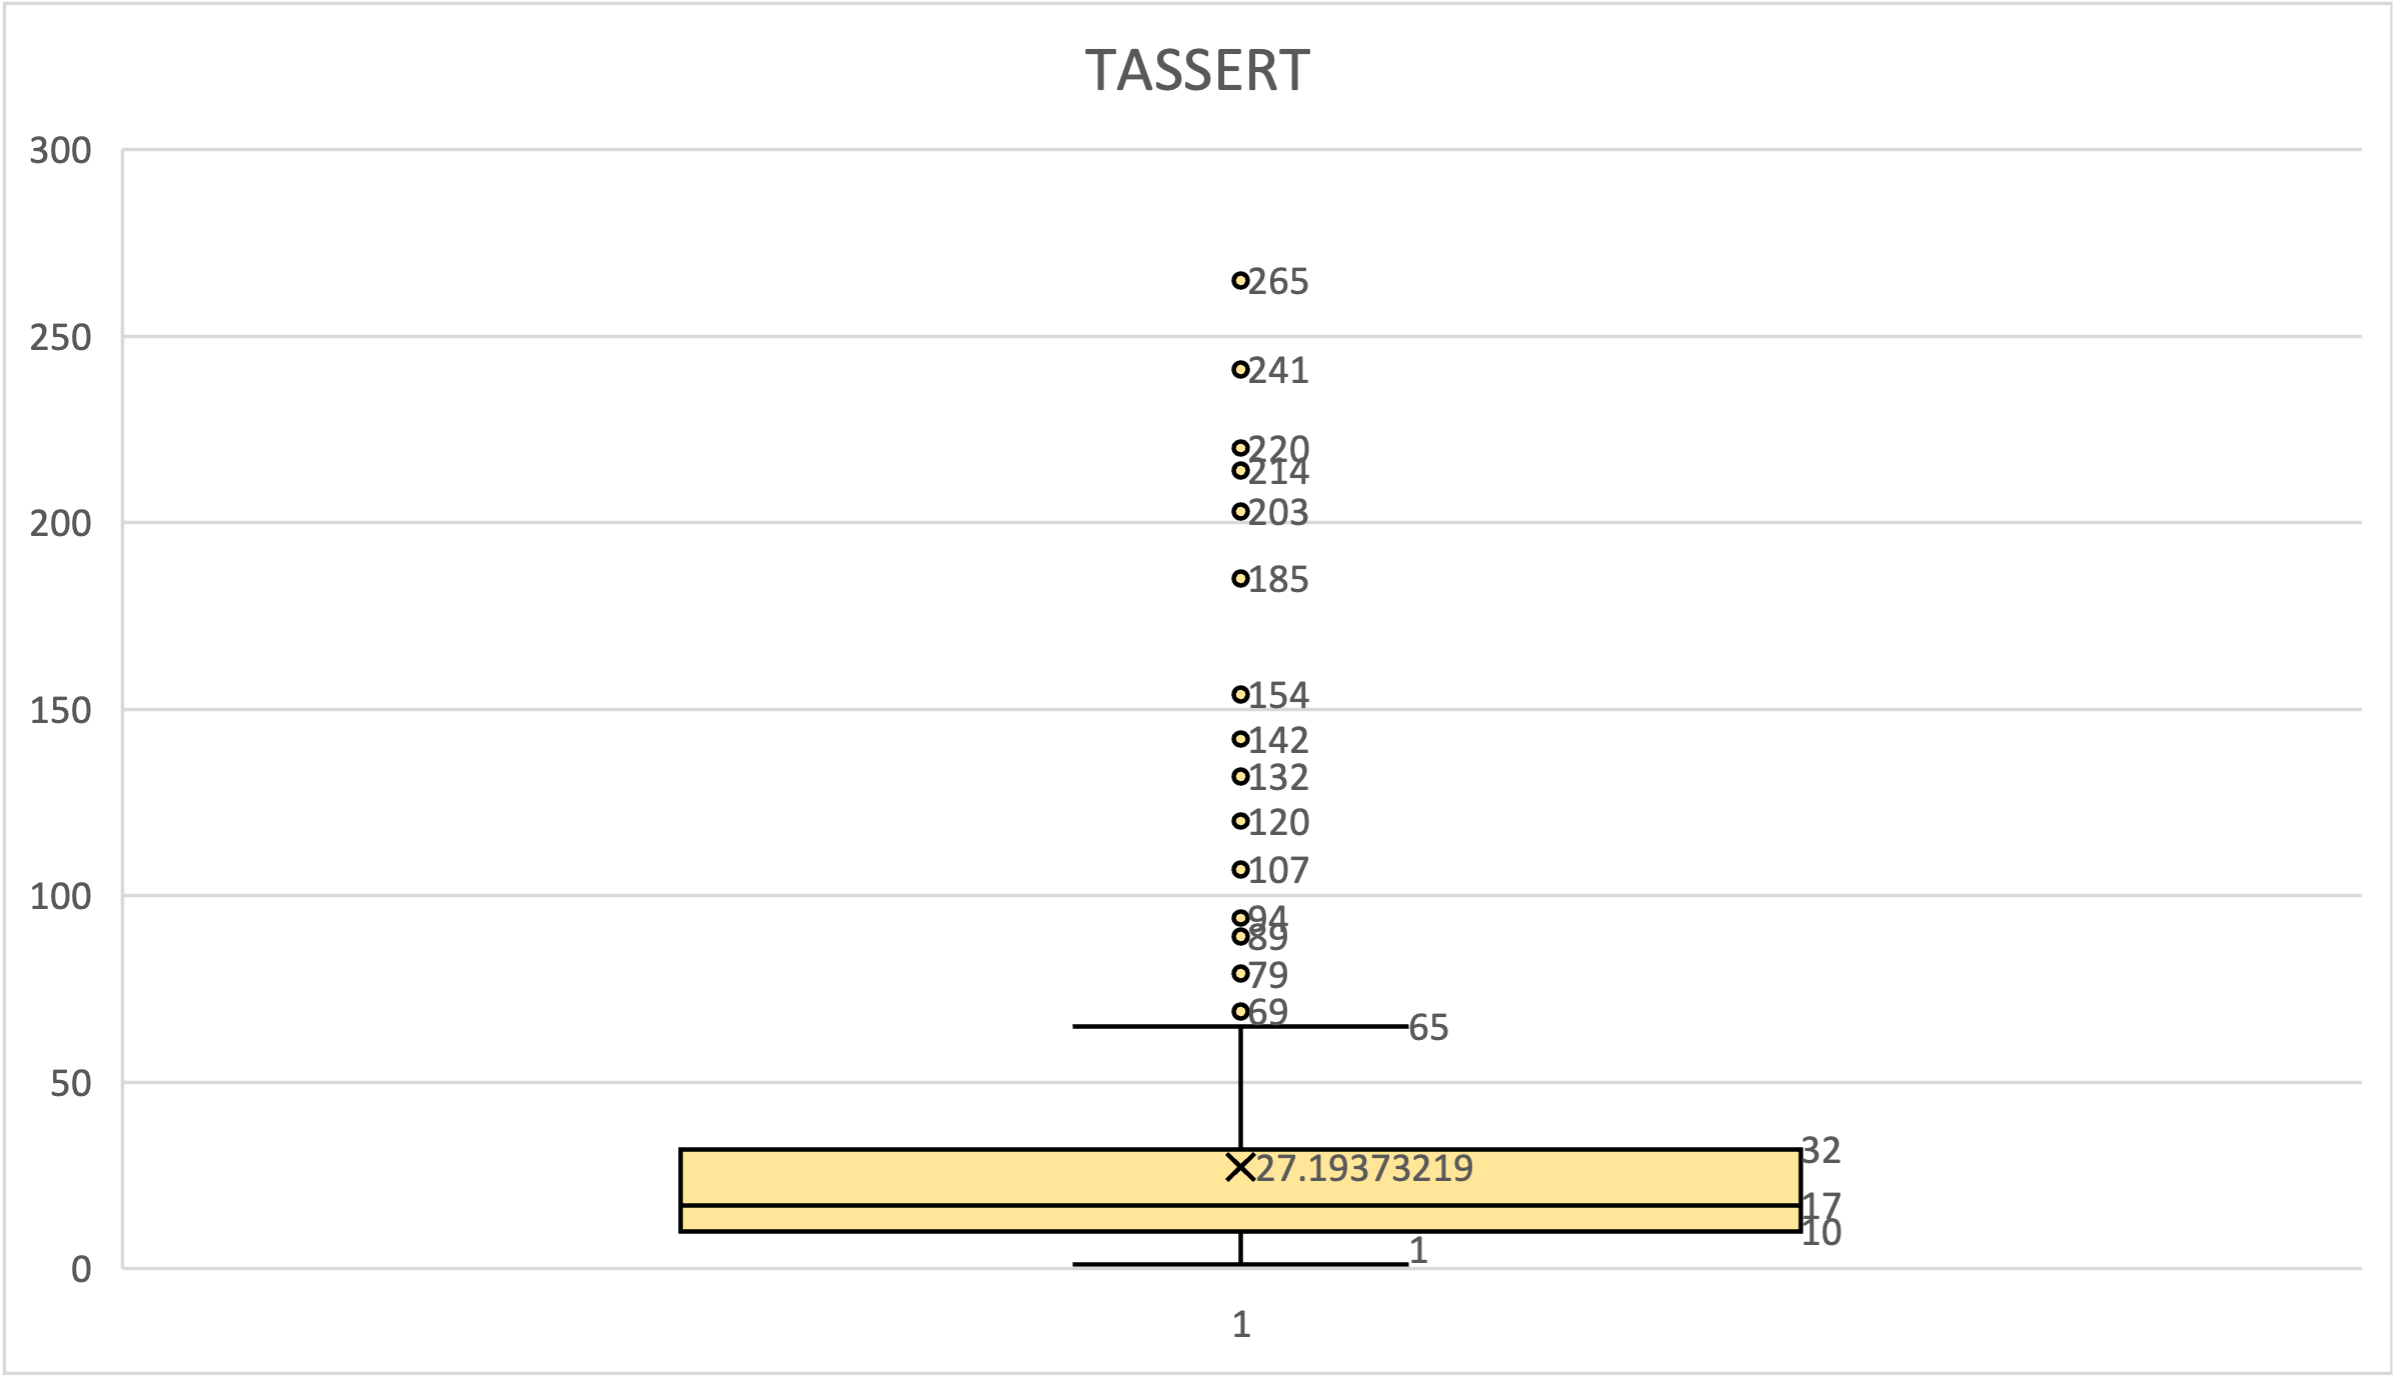
\includegraphics[width=0.5\textwidth]{images/TASSERT.png}
    \caption{Boîte à moustaches WMC}
    \label{fig:TASSERT.png}
    \end{figure}
\end{itemize}


\subsection{Analyse des Résultats}
% Description des informations pertinentes extraites des boîtes à moustaches (médiane, etc.)
À partir de nos données et graphiques obtenus, nous pouvons savoir

TLOC: 
Sa médiane est de 83, indiquant la tendance centrale de l'ensemble de données;
La longueur de la boîte est de 78. On peut savoir que le nombre de lignes de code dans les 50 \% du milieu du fichier est réparti entre 47-125.
La limite supérieure est de 242, ce qui signifie que si le nombre de lignes de code dans un fichier dépasse cette valeur, il peut être considéré comme une valeur aberrante.
Sa limite inférieure est -70, ce qui est un nombre négatif. Il n'a aucune signification de référence car le nombre de lignes de code ne peut pas être négatif.

WMC:
La médiane est de 9 et la longueur de la case est de 4, ce qui indique que le nombre de méthodes dans la plupart des classes est relativement concentré et que les changements ne sont pas évidents.
la limite supérieure est 18. Si la valeur d'un fichier dépasse 18, cela indique que certaines classes ont un nombre inhabituellement élevé de méthodes.
La limite inférieure est de 2, ce qui signifie que peu de classes ont très peu ou pas de méthodes.

TASSERT:
La médiane est de 17. Reflète le nombre d'assertions couramment utilisées dans les tests de fichiers
La longueur de la boîte est de 22, ce qui montre que le nombre d'assertions est relativement réparti dans l'ensemble de données.
La limite supérieure est de 65. Si elle dépasse cette valeur, cela signifie que certains cas de tests utilisent beaucoup de falaises.
La limite inférieure est de -23, ce qui est la même que dans le cas TLOC. C'est également une valeur de référence dénuée de sens car le nombre d'assertions ne peut pas être négative.

Conclusion,
Complexité du code: la méthode de distribution large de TLOC signifie que le nombre de lignes de code dans les fichiers de test varie considérablement, certains ont plus de lignes et d'autres moins.
Conception des classes: la longueur courte de la boîte de WMC indique que la complexité de la plupart des classes est relativement cohérente et ne fluctue pas beaucoup.
Cas de test: la plus grande longueur de la boîte de TASSERT indique que l'utilisation des assertions varie considérablement entre les différents cas de test.


\section{Tâche 2: Étude des Corrélations avec Python}
\subsection{Vérification de la Normalité des Données}
% Description de l'utilisation du test de Shapiro-Wilk pour vérifier la normalité
% Inclusion des résultats du test de normalité
Nous avons utilisé le test de Shapiro-Wilk \cite{SHAPIRO1965} en Python pour vérifier la normalité des données. Les résultats montrent que toutes les métriques (TLOC, WMC, TASSERT) ne suivent pas une distribution normale avec une p-valeur inférieure (ici $<<<$) à 0,05. Nous avons utilisé les librairies pandas \cite{reback2020pandas} et shapiro (scipy.stats) \cite{2020SciPy-NMeth} pour trouver nos données.
\\\\
Voici les valeurs obtenues. \\(Note: ND signifie normally distributed):

\begin{figure}[H]
    \centering
    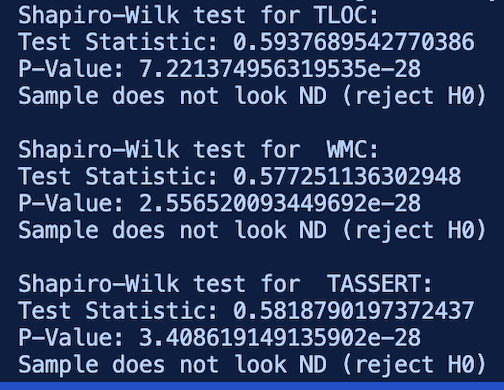
\includegraphics[width=0.5\textwidth]{images/shapiro-wilk.png}
    \caption{Test de normalité Shapiro-Wilkin.}
    \label{fig:Test de normalité Shapiro-Wilkin}
\end{figure}


\subsection{Calcul des Coefficients de Corrélation}
% Description du calcul des coefficients de corrélation entre TLOC, WMC et TASSERT avec Python
Les coefficients de corrélation entre TLOC, WMC et TASSERT sont les suivants :\\
\begin{itemize}

    \item \textbf{Corrélation entre TLOC et TASSERT} : \\Spearman Rank Correlation Coefficient: 0.834606519587501 \\
P-Value: 2.1276357013448774e-92
    \item  \textbf{Corrélation entre WMC et TASSERT} :\\ Spearman Rank Correlation Coefficient: 0.6149330438016306\\
P-Value: 6.893133521020008e-38
\end{itemize}
\subsection{Régression}
Afin d'effectuer la régression, nous avons utilisé un script Python avec les librairies pandas \cite{reback2020pandas}, numpy \cite{harris2020array}, matplotlib.pyplot \cite{Hunter:2007}afin de dessiner des 'best fit line' (en rouge) - c'est à dire les lignes représentant nos équations - et compare avec nos données (en bleu). Voici un visuel des 2 droites ainsi que l'équation de nos droites de régression linéaire.\\
\begin{itemize}
    \item  \textbf{Equation TLOC(x) et TASSERT(y)} : \\y = 0.251790600546902 * x + -1.6764188502983188
    \begin{figure}[H]
    \centering
    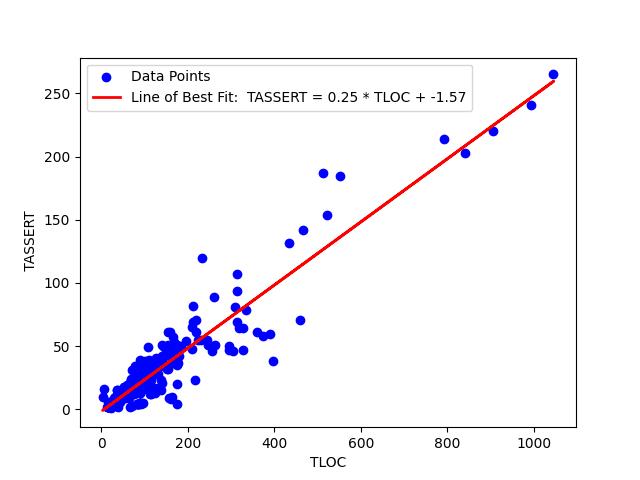
\includegraphics[width=0.6\textwidth]{images/tassert_tloc.png}
    \caption{Régression TLOC-TASSERT}
    \label{fig:Régression TLOC-TASSERT}
\end{figure}
    \item  \textbf{Equation WMC(x) et TASSERT(y)} : \\y = 4.404718600470233 * x + -21.699130611226817
   
    \begin{figure}[H]
    \centering
    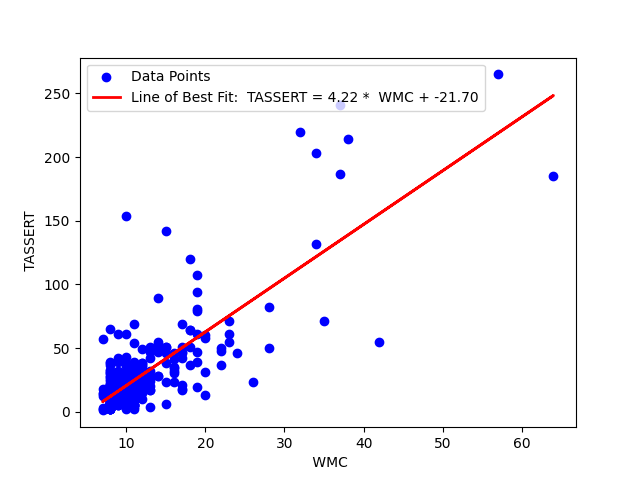
\includegraphics[width=0.6\textwidth]{images/tassert_wmc.png}
    \caption{Régression WMC-TASSERT}
    \label{fig:Régression WMC-TASSERT}
\end{figure}
\end{itemize}



\subsection{Analyse de la Tâche 2}

Dans le cadre de la Tâche 2, notre objectif était d'étudier les corrélations entre les métriques TLOC, WMC et TASSERT. Nous avons suivi les étapes suivantes :
\\\\
\textbf{Vérification de la Normalité des Données}\\
Avant d'entreprendre une analyse de corrélation, nous avons effectué un test de normalité (Shapiro-Wilk) sur nos données pour déterminer si elles suivaient une distribution normale. Les résultats ont montré que \textit{les données ne sont pas normalement distribuées.}

Cela indique que nos données ne suivent pas une distribution gaussienne, ce qui est un prérequis pour certains tests statistiques paramétriques. Par conséquent, nous avons opté pour des méthodes de corrélation non paramétriques.
\\\\
\textbf{Calcul des Coefficients de Corrélation}
Nous avons utilisé le coefficient de corrélation de Spearman, un test non paramétrique approprié pour les données non normalement distribuées, afin d'évaluer les relations entre les métriques.
\\\\
Les résultats des corrélations sont les suivants :
\begin{itemize}
\item \textbf{TLOC et TASSERT :} Une corrélation positive significative a été observée, avec un coefficient de Spearman de 0.83. Cela suggère une forte corrélation entre le nombre de lignes de code et le nombre d'assertions dans les classes.
\item \textbf{WMC et TASSERT :} Une corrélation positive moins forte, mais toujours significative, a été trouvée, avec un coefficient de Spearman de 0.61. Cela suggère une corrélation moins forte entre le nombre de méthodes pondérées par classe et le nombre d'assertions.
\end{itemize}

\textbf{Régression}\\
Nous avons également réalisé des analyses de régression pour modéliser les relations entre les métriques. Les équations des droites de régression ont été obtenues, montrant comment les variables évoluent les unes par rapport aux autres.
\\
\begin{itemize}
\item \textbf{TLOC et TASSERT :} L'équation de régression indique qu'il existe une relation linéaire positive entre le nombre de lignes de code et le nombre d'assertions, avec une pente de 0.25.
\item \textbf{WMC et TASSERT :} L'équation de régression montre une relation linéaire positive moins forte entre le nombre de méthodes pondérées par classe et le nombre d'assertions, avec une pente de 4.40.
\end{itemize}

\textbf{Interprétation}\\
Ces résultats suggèrent que les classes avec un nombre élevé de lignes de code ont tendance à avoir un nombre plus élevé d'assertions. De plus, bien que la corrélation entre le nombre de méthodes pondérées par classe et le nombre d'assertions soit positive, elle est moins forte que la corrélation observée avec le nombre de lignes de code.


\section{Tâche 3: Évaluation de l'Hypothèse}

\subsection{Conception de l'Expérience}
% Description de la conception de l'expérience pour évaluer l'hypothèse
Nous choisissons une approche hypothético-déductive pour tester l'association entre le nombre d'assertions et la complexité des classes.

\subsection{Énoncé des Hypothèses}
% Description de l'hypothèse
Hypothèse nulle (H0): Aucune augmentation de complexité pour les classes avec plus de 20 assertions par rapport à celles avec moins.\\Hypothèse alternative (H1): Les classes avec plus de 20 assertions sont plus complexes.

\subsection{Définition des Variables}
% Description des variables
Variable Indépendante: Nombre d'assertions (plus grand ou égale 20 ou plus petit que 20).
\\  Variables Dépendantes: Mesures de complexité TLOC et WMC
\subsection{Présentation des Résultats}
% Présentation des résultats de l'expérience et leur interprétation
Les données représentées dans les boîtes à moustaches pour TLOC, WMC et TASSERT montrent une distribution avec des écarts importants par rapport à la normale, indiquées par la présence de plusieurs valeurs extrêmes, ce qui est également étayée par le test de Shapiro-Wilk. Et la médiane pour TASSERT est relativement élevée. Les corrélations de Spearman confirment une association positive entre TASSERT et les mesures de complexité.

\section{Conclusion}
% Résumé des principales conclusions de l'étude
La présence de fortes corrélations et les distributions observées dans les boîtes à moustaches suggèrent que les classes avec un nombre plus élevé d'assertions tendent à avoir des mesures de complexité plus élevées, ce qui appuie l'hypothèse alternative H1.

\section{Discussion des Menaces à la Validité}
% Discussion des possibles menaces à la validité de l'expérience
 Les corrélations ne prouvent pas la causalité et les boîtes à moustaches révèlent la variabilité des données. D'autres facteurs peuvent influencer la complexité des classes.

\section{Références}
\bibliographystyle{plain}
\bibliography{references}  

\end{itemize}
\end{document}

